\documentclass[]{article}

\usepackage{amsmath}
\usepackage[]{graphicx}
\usepackage{subfigure}
\usepackage[latin1]{inputenc}
\usepackage{comment}
\usepackage{url}
%\usepackage{biblatex} 
%\usepackage[pdftex]{graphicx}
\usepackage{anysize}
\marginsize{3cm}{3cm}{2cm}{2.5cm}%l r t b

\title{Using an Open source face tracker for identity detection and facial expression Recognition}
%\title{Controlling a smart phone using gaze gestures}
%\title{Gaze gestures as an innovative HCI method for smartphone like devices}
 
\author{Eduardo Neiva, Jesus Nuevo, David Rozado}

\setlength\parindent{0pt} %no indentation in paragraphs
% Document starts
\begin{document}

\maketitle

\section{Abstract}
Face and eye tracking technology are fairly well developed and robust technologies. Eye tracking in combination with
gaze estimation permits the monitoring of the user's area of attention on a computer screen while also providing a hint
about possible intention. Facial tracking can augment eye tracking by monitoring facial features that can convey the
identity of the user or its internal cognitive state as expressed through its facial expression. In this work, we use an
open source face tracker that can recognize and classify facial expressions from continuous video input. The system uses
---------- for jesus to fill --------------. We show that the face tracker is a powerful tool to recognize the identity
of the user among a large pool of subjects. We also show that it can robustly recognize facial expressions of users on
which the system has been trained while also performing well on users never exposed before to the system. This positive
results and the open source nature of the system suggest the advantages of augmenting traditional eye trackers by
combining them with face tracking algorithms as the one suggested to enrich the set of features available to monitor a
human while interacting with a computer.


\section{Introduction}
Traditional Human Computer Interaction (HCI) could be augmented by providing computer systems with the ability to
recognize the emotions of the humans interfacing them. Emotions are conveyed by humans  using the visual, vocal
and other physiological means such as body gestures. Facial expressions are an indirect proxy to measure the internal
cognitive emotions of humans. Impaired facial expression recognition by humans can be a sign of serious cognitive
dysfunction such as schizophrenia \cite{Edwards2002789}.  Facial attributes can be tracked computationally through a
video stream of the subject's face. Making the computer aware of the emotions of the user could lead the way towards
more natural in fluid forms of interaction.


In this work we describe the usage of an open-source face tracker to feed a set of machine learning classifiers striving
to identify subjects identity and their facial expressions. The face tracker provides a set of invariant features
extracted from the tracked faces (MAYBE JESUS COULD COMPLETE THIS). We used support vector machines 
to classify the invariant features provided by the face tracker.


The psychological literature has traditionally classified facial expressions in seven categories: neutral, anger, disgust, fear,
joy, sadness and surprise. in these experiments, we use some additional facial gestures such as: raising eyebrows and open mouth.
(EDUARDO PLEASE COMPLETE THIS LIST with the accurate info).


Researchers have employed a variety of methods to carry out facial expression recognition such as optical flow
computation  and symbolic representations \cite{Yacoob506414}, local binary patterns \cite{Shan2009803},  Bayesian
network classifiers \cite{Cohen1211408}, geometric deformation features and support vector machines
\cite{kotsia4032815}, hidden Markov models \cite{aleksic1597130, Cohen2003160}, Parametric flow models
\cite{blackAndYacoob}, AdaBoost and linear discriminant analysis \cite{bartlett1398364}. The surveys from
\cite{bartlett1398364} and \cite{Fasel2003259} are two good review sources about machine learning methods 
for fully automatic recognition of facial expressions. 


Previous work has employed a variety of techniques to classify  facial expressions. The work from \cite{Cohen2003160}
tested the classic neural network classifiers for classifying expression from video, focusing on changes in distribution
assumptions and feature dependency structures. Authors also proposed an tested the architecture of Hidden Markov Models
(HMM) for automatically segmenting and recognizing human facial expressions. Authors reported recognition rates up to
83\% For frame-based recognition methods and 82\% for the multilevel HMM.
 


The work from \cite{Chen670976} investigated the emotional contents of speech and video based facial expression to
proposes a bioinspired algorithm for human facial expression recognition, concluding that both modalities can be
complimentary and able to achieve higher recognition rates than either modality alone. Authors in \cite{Busso:2004} also
used a multimodal approach to combine acoustic information and facial expression analysis in order to detect human
emotions. In their work, authors demonstrated that when both modalities are fused, the performance and the robustness of
the emotion recognition system improves considerably.


Authors in \cite{Bartlett4624313} used perceptual primitives to code seven facial expressions in real-time. Their system
first detects frontal faces using a cascade of feature detectors trained with boosting techniques. The expression
recognizer receives image patches located by the phase detector. A Gabor representation of the parts is used  by a bank
of kernel based classifiers. Authors used a combination of Adaboost and support vector machines to enhance performance.
One of the most interesting properties of this work was its ability to change the outputs of the classifiers smoothly
as a function of time, hence, providing a dynamical representation of facial expression.


The work from \cite{lijunyin} deviates from the typical 2D static image or 2D the video sequence recognition of
facial expression arguing that that a 2D-based analyses is incapable of handling large pose variations and proposing
instead the usage of classification techniques on 3-D facial expression models and making available to the community a
database of prototypical 3D facial expression shapes.

 
The work from \cite{Cohn840611} made available over 2000 digitized image sequences from  182 adult subjects of
varying ethnicity, performing multiple tokens of most primary facial expressions to create a comprehensive testbed for
comparative studies of facial expression analysis.


Facial identity recognition is another subject that has drawn a lot of attention in the research literature. While being
apparently trivial for humans to solve, automatic approaches have traditionally lagged behind the performance of humans
by at least one order of magnitude in terms of recognition performance. These approaches have only recently started to
catch up with the ability of the human brain to recognize faces \cite{onintelligence, Rozado2012b}. Face recognition is
important  for a wide range of commercial and law enforcement applications. Only recently has the technology required to
carry out automatic classification of faces become available. But the recognition of faces in outdoor environments 
where variation in pose and illumination are continuous remains a largely unsolved problem.

The work from \cite{Zhao:2003} provides a good literature survey on the subject of face recognition. In
\cite{Craw1987183}, authors undertake an in-depth discussion of face features automatic extraction for classification purposes of
grayscale images.

The work from \cite{Zhang20092876} undertakes a comprehensive review  of the challenging topic of pose invariant face
recognition, and while showing that the performance of different methods is still far from perfect, several promising
directions for future research  are suggested.

Authors in \cite{Tan20061725} review the also challenging topic of face recognition using  just one image per
class for training comparing several prominent algorithms for the tasks. the rationale for the study is the reported
critique that several face recognition techniques rely heavily on the size of the training set.

(i NEED TO COMPLETE THE LITERATURE REVIEW FOR IDENTITY RECOGNITION)

In summary, in this paper we apply that open source face tracker XXXXX for identity recognition and for facial
expression recognition. We suggest that facial tracking can be a powerful complement to traditional eye tracking  by
augmenting the set of features being tracked during human computer interaction. This  can potentially allow computer
systems to more precisely recognize the cognitive state of the human interfacing them through the proxy features of facial
dynamics.


\section{Methodology}
(eDUARDO IT IS VERY IMPORTANT THAT THE THE SECTION YOU INCLUDE A BRIEF subsection OF JUST ONE PARAGRAPH IN WHICH YOU
PROVIDE A BRIEF DESCRIPTION OF WHAT SUPPORT VECTOR MACHINES ARE)

\subsection{SVM}

Support vector machines have become popular in the supervised learning models
for classification. It generates a set of hyperplanes in a multiple dimensional
space which is used for classification.  A good classification is produced by
maximizing the distances between the nearest training data points of the classes.

Whenever this problem is not linearly separable in that space, a technique named
kernel functions was stated to map the original space into a much
higher-dimensional space in order to achieve easier separations. Since SVM makes
binary decision, a multi-class one-to-one classification was assigned for the problem.
In the following experiments, it was used an open source SVM library called
LIBSVM, it�s available for many languages and support most of the needs on the
SVM classification.

ADD REFERENCE FOR THE LIBSVM



\subsection{Face Tracker}
---- For Jesus to fill in---------------

\subsection{Experimental Setup}
The dataset that was used to train and test the recognition algorithms was specifically generated for this work. It
consists of 50 people (age distribution ranged from 19 to 40 years old). From the entire set, 80\% were male, 16\% were
Latino and 10\% were Asian. The data extraction was made using a standard notebook webcam, 1.3 MP, running at a
resolution of 640x480. The distance between the camera and the subject's face was about 114cm. The data extracted from
the face tracker was a vector with 24 dimensions that represents a particular face shape at any given time point. This
vector has the property of being invariant within a particular face shape.
(i DON'T LIKE THE LAST SENTENCE, MAYBE jESUS COULD IMPROVE OR ADD SOMETHING so it makes better SENSE)

\subsubsection{Metodology of the data extraction}
Every participant involved in the experiment was asked to perform eleven different facial shapes or expressions.
Five of them were stereotypical emotion common to every person (i.e., neutral, anger, disgust, fear, happiness,
surprise). The remaining facial expressions where: open mouth, raised eyebrows,
kissing face, closed smile, squint face.

Even though the feature vector produced  by the face tracker was invariant to changes in scale, the distance
between the camera and the subject was kept constant to maintain uniformity during the data collection.

The data collection was divided in two phases, the training and the capturing. The training was the phase in which the
subject was told to perform every face shape in order to practice how to perform each of the requested face
representations.

The capturing phase consisted on the subject representing them again and the computer system recording these instances
for subsequent training and validation. 

\begin{figure}[ht]
\begin{center}
\vspace{-3mm}
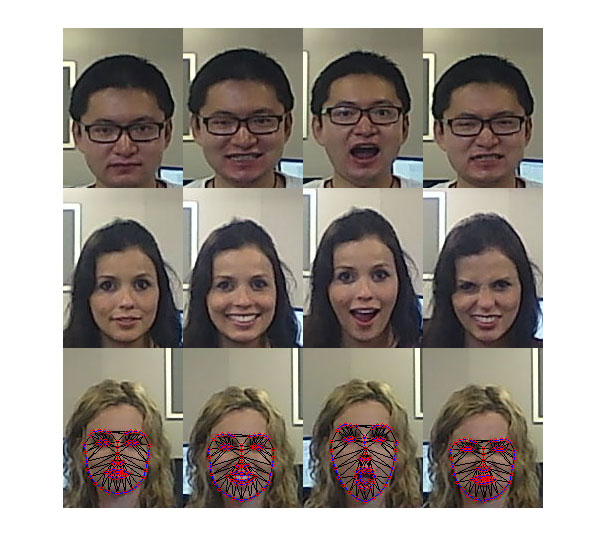
\includegraphics[width=0.95\textwidth,height=70mm]{figures/dataExtrationExamples.jpg}
\end{center}
\caption{\textbf{Data extraction} Samples of the face shapes recorded.}
\label{figureLabel}
\end{figure}

For every face shape recorded, 20 samples were recorded with a small time
interval between them (less than one second). Each sample consists on recording
the invariant vector that transforms a neutral face shape into the deformed
face shape that fits the subject facial expression. Since there was fluctuations on the borders
of the face shape tracker and this generated some instability on the
invariant vector, 20 samples to smooth out this error.

During the data extraction period, we observed that every person had a unique invariant vector signature which was
specific for each facial expression on for different persons. We thought that this invariant feature vector could be
used to recognize people as well as data facial expressions. The invariant feature vector specific for each person and
facial expression can be seen in the Figure \ref{comparationBetweenFaces}.

For the task of facial expression recognition, even though every person has its own unique feature vector signature for
each face expression, there is a similarity between these vectors when comparing the same face shape of different
people, thus the goal of the SVM was to generate an abstraction of each facial expression class in order to be able to
carry out facial expression classification.

\subsubsection{Data training}

The first experiment tried to recognize people's identity using the entire data
set of the study participants. Three methods of training was used for this
experiment.
\begin{description}
\item[$\bullet$ Method 1:]Only the neutral face shape was used in this
experiment.  The training and test set data were generated by splitting 70\% of
the samples of each person to train and the remaining to test. The procedure is
conducted by increasing the number of people in the experiment and testing the 
results accuracy.
\item[$\bullet$ Method 2:]Six face shapes were used in this experiment (neutral,
opened mouth, smiling, raised eyebrow, surprise and anger face). All of those
shapes were transformed into a unique class that corresponds to the participant.
he training and test set data were generated by splitting 70\% of the samples of
each person to train and the remaining to test. The procedure is conducted by
increasing the number of people in the experiment and testing the results
accuracy.
\item[$\bullet$ Method 3:]All the face shapes were used in this experiment. All
those face shapes of one person were transformed into a unique class. The
training and test set data were generated by splitting 70\% of the samples of
each face shape to train and the remaining to test. The procedure is conducted
by increasing the number of people in the experiment and testing the results
accuracy.
\end{description}

For face shape recognition, there were three different methods of training that
were used throughout the experiments. All of them used a 7:3 ratio for testing 
and training set respectively.

\begin{description}
\item[$\bullet$ Method 4:] All facial expression were used in this experiment,
the training and test set share the same group of participants but using
different  versions( captured in a different time slot) of the same face shape
for training and testing. The ratio is kept by assigning 70\% of the face shapes
of this person to the train set and 30\% to the test set. The procedure is conducted
by increasing the number of people in the experiment and testing the results
accuracy.
\item[$\bullet$ Method 5:] All facial expressions were used in this experiment,
the training and test set don�t  share the same group of participants, the ratio
is kept by assigning 70\% of the people on the training set and 30\% on the
test set. The procedure is conducted by increasing the number of people in the
experiment and testing the results accuracy.
\item[$\bullet$ Method 6:] The third method had a different methodology, it was
used the all the participants but its goal was to analyze the impact on accuracy
on increasing the number of face shapes.  The training and test set don�t share 
the same group of people, and the ratio was to assign 70\% of the whole set to
train and 30\% to test. The procedure is conducted by increasing the number of
face shapes (classes) in the experiment and testing the results accuracy.
\end{description}

\begin{figure}[ht]
\begin{center}
\vspace{-3mm}
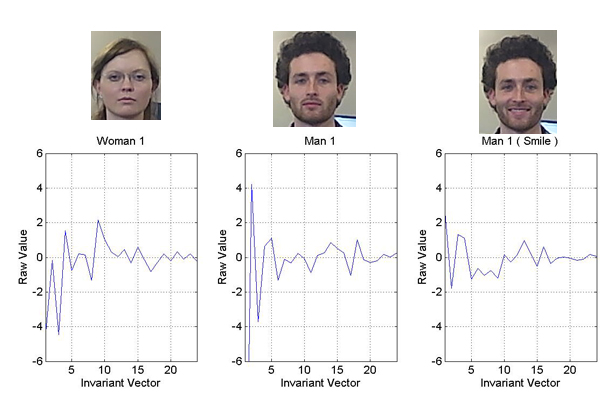
\includegraphics[width=0.95\textwidth,height=75mm]{figures/comparationBetweenFaces2.jpg}
\end{center}
\caption{\textbf{Invariant and Unique Feature Vectors of Facial Expressions.} this figure displays a. Typical feature 
vector signature specific for a given person. These constraint can be used to recognize people. The feature vector
provided by the face tracker changes for each facial expression perform but remains invariant we seen a given facial 
expression. Furthermore, features vectors of the same facial expression among different people share commonalities that
can be exploited to carry out facial expression recognition among different people.}
\label{comparationBetweenFaces}
\end{figure}s

\section{Results}


 eDUARDO HERE YOU NEED TO EXPLAIN THE SPECIFICS OF THESE EXPERIMENTS, where you using ALL
FACIAL EXPRESSIONS OR JUST NEUTRAL? what is THE FRIENDS BETWEEN the labels in the figure including and excluding?).

\begin{figure}[ht]
\begin{center}
\vspace{-3mm}
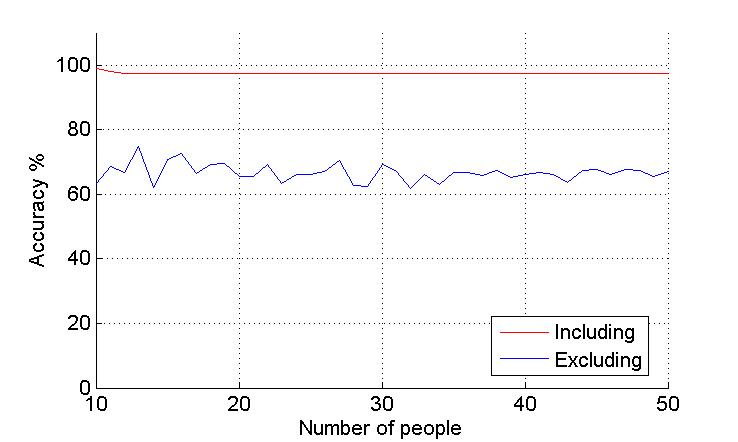
\includegraphics[width=0.95\textwidth]{figures/figureRecognizeFacialExpression5.jpg}
\end{center}
\caption{\textbf{Identity Recognition Results} Explanation of the figure.}
\label{identityRecognition}
\end{figure}

\subsection{Recognizing Face Expressions}

In this experiment, the goal was to recognize each of the 11 different classes
of facial expressions in the training set. It was used all the 24 features of
each face shape. It was given two different aproaches on the results
measurement. These different approaches are described by the Method 4 and
Method 5 in the Data training section.
For the first method, since the group of people used in the training set is the
same that it is used on the test set, and even though the data used in the test
set was different compared to the training set, it was expected to have high
accuracy results.
For the second method ( Method 5), it was expected that as long as it is
increased the number of people in the data, the accuracy gradually would increase.
 
###STOPPPED HERE

The results of the facial expression recognition  are shown in Figure
\ref{identityRecognition}.
 
\subsection{Recognizing Face Expressions increasing the number of classes}

Using a 10-fold cross validation, in this approach the goal was to measure the
change of effiency of the algorithm by increasing the number of classes from 2
to 11. The amount of people used was 50.

\begin{figure}[ht]
\begin{center}
\vspace{-3mm}
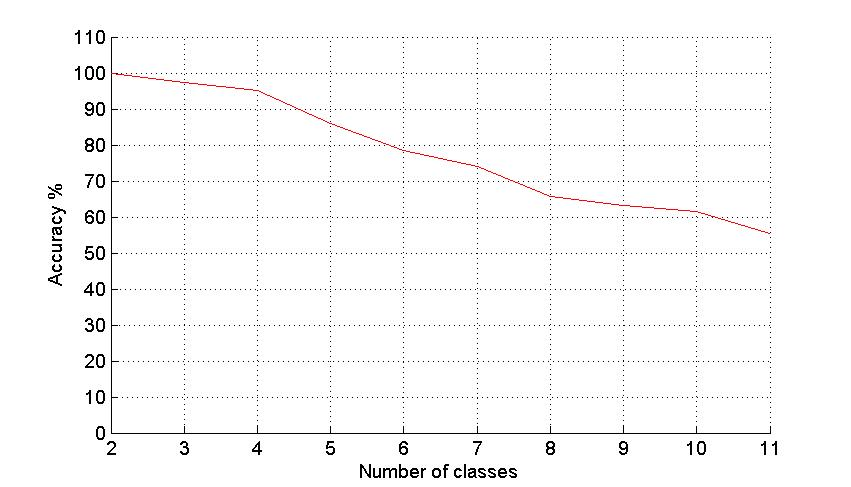
\includegraphics[width=0.95\textwidth]{figures/50people_increasing_classes.jpg}
\end{center}
\caption{\textbf{Effect of Increasing the Number of Facial Expressions to Recognize} Explanation of the figure.}
\label{increasingNumberExpressions}
\end{figure}

Figure \ref{feRecognition} shows the results of increasing the number of people
to be recognized by the classifier.

\subsection{Recognizing People}

In the third approach, there is a change on what are the classes of the
algorithm. Instead of face shapes being the classes, in this method, the people
to recognize were transformed into the classes. Therefore, the increase of
people to recognize increase the number of the classes, thus decreasing the
efectiviness of the algorithm. It was analysed from 2 to 50 people the algorithm
accuracy. It was also analysed in three different scenarios, using only the
normal face shape, using only 6 and using all 11 face shapes in each classe.
 


\begin{figure}[ht]
\begin{center}
\vspace{-3mm}
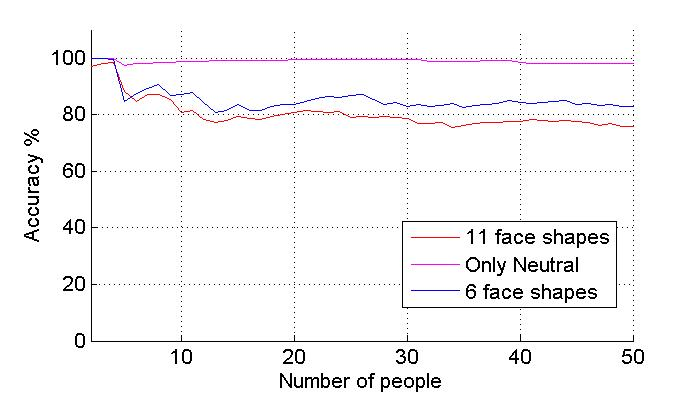
\includegraphics[width=0.95\textwidth]{figures/peopleRecognition4.jpg}
\end{center}
\caption{\textbf{Facial Expression Recognition Results} Explanation of the figure.}
\label{feRecognition}
\end{figure}


Figure \ref{feRecognition} shows the results of increasing the number of people
to recognize facial expressions


\section{Discussion}
In this work we have used an open-source face tracker to recognize facial identity and to classify facial expressions.


\bibliographystyle{plain}
\bibliography{library}

\end{document}
